\documentclass{article}
\usepackage{tabularx}
\usepackage{amsmath}
\usepackage{graphicx}
\usepackage[top = 2cm, bottom = 2cm, right = 2cm, left = 2cm]{geometry}
\usepackage{cite}
\usepackage[final]{hyperref}
\usepackage{listings}
\hypersetup{
	colorlinks=true,
	linkcolor=blue,
	citecolor=blue,
	filecolor=magenta,
	urlcolor=blue         
}

\begin{document}

\title{Practicle 5\\Debugging a CUDA application}
\date{30/01/19}
\maketitle

\begin{abstract}
	
\end{abstract}

\section{Nsight}
Nsight is a development environement for CUDA. This tool is integrated into Visual Studio. When you run you program through Nsight you can reach breakpoint into your kernel. Frist you need to specify your application to generate GPU Debug Information. Go to the Property panel of your project and go on the Device section of CUDA C/C++. Here you can enable the Generate GPU Debug Information (Yes (-G)). Now we can use breakpoint into our kernel. Put one breakpoint after the index computation and run your program. You can read in debug mode the value of your index for the first thread of the first block.
\subsection{Warp Info}
Most of the time debug only the first thread solve problem because we use SIMD architecture. However, if there is a branch in the kernel you may want to debug another thread. On the Nsight panel, open Windows/Warp Info.

\begin{figure}[h]
	\centering
	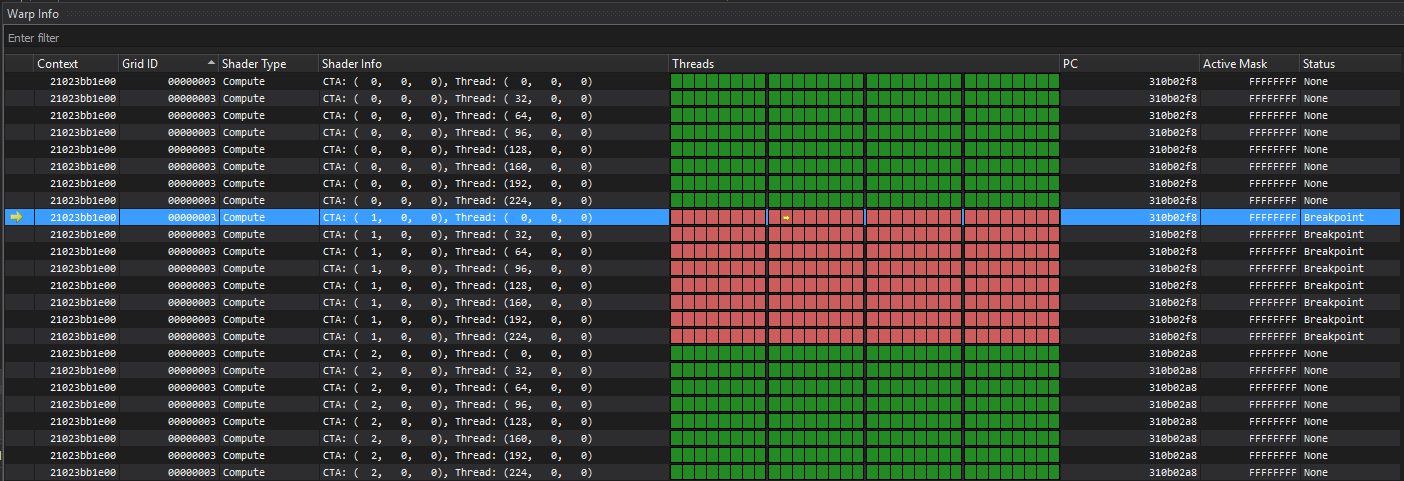
\includegraphics[scale=0.47]{figures/warpinfo.png}
	\caption{Warp Info}
\end{figure}

You can see several color infos for each warps. If it is red is beause the execution reach the breakpoint. If it is green it's mean the thread is active. There is 8 threads states.

\begin{figure}[h]
	\centering
	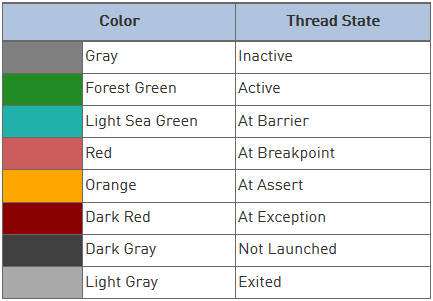
\includegraphics[scale=0.6]{figures/threadstate.png}
	\caption{Warp Info}
\end{figure}

\newpage
\subsection{Lanes}
The lane section allow us to debug threads for the active warp. We can find the same informations as the warp info. If you change the current warp on the warp info it will impact this window too.
\begin{figure}[h]
	\centering
	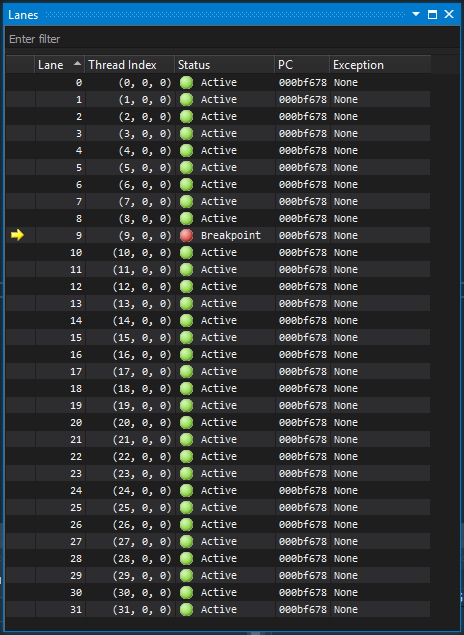
\includegraphics[scale=0.6]{figures/lanes.png}
	\caption{Warp Info}
\end{figure}

\newpage
\subsection{GPU Registers}
Sometime you may need to see the disassembly code for debugging (Right clic on your code/Go to disassembly). You can fallow the value stored into the GPU register on this last window.

\begin{figure}[h]
	\centering
	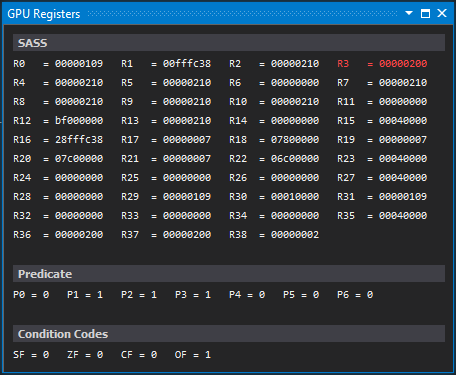
\includegraphics[scale=0.6]{figures/register.png}
	\caption{Warp Info}
\end{figure}

\newpage
\section{Test limits of your program}
We see on the last practical how to grab an error. Now we'll try to get errors. Create a recursive function called 100 times and look at the error throwed. It is because you don't have enought memory for your stack. You can get your device stack size in this way:
\begin{lstlisting}
	size_t value;
	cudaDeviceGetLimit(&value, cudaLimitStackSize);
\end{lstlisting}
And if you want to modify this limite just call:
\begin{lstlisting}
	cudaDeviceSetLimit(cudaLimitStackSize, value);
\end{lstlisting}

\end{document}